% ===================================================================
% Preprint Title: A 3D Mathematical Model of a Dynamically Coupled Field...
% Author: Toshiya Konno
% Version: 4.0 Final Manuscript (Date: 2025-07-23)
% This is the definitive final version, with only the caption for Fig S3
% being updated as per the final review. No other changes have been made.
% ===================================================================

\documentclass[a4paper,11pt,ja=standard,lualatex]{bxjsarticle}

% ---------- Packages (Reverted to v3.0 configuration) ----------
\usepackage{fontspec}
\usepackage{amsmath,amssymb,amsfonts}
\usepackage{graphicx}
\usepackage{geometry}
\usepackage{hyperref}
\usepackage{authblk}
\usepackage{placeins}
\usepackage{caption}
\usepackage{unicode-math} 

% ---------- PDF Metadata ----------
\hypersetup{
  pdftitle={A 3D Mathematical Model of a Dynamically Coupled Field Inspired by Operator Algebras (Version 4.0)},
  pdfauthor={Toshiya Konno},
  pdfsubject={We extend our quantum-classical hybrid model to include thermal fluctuations. This reveals a novel dynamical equilibrium, a "Thermally Excited Oscillatory State," and provides quantitative evidence of stochastic resonance.},
  pdfkeywords={Coupled Gross–Pitaevskii Equations; Quantum-Classical Hybrid System; Tensegrity; Soliton Dynamics; Topological Robustness; Dissipation; Phase Transition; Thermal Fluctuation; Stochastic Resonance},
  pdfcreator={XeLaTeX (TeX Live)},
  pdflang={en}
}

% ---------- Fonts & Math Fonts ----------
\setmainfont{TeX Gyre Termes}
\setjamainfont{IPAexMincho}
\setsansfont{IPAexGothic}
\setmathfont{TeX Gyre Termes Math}

% ★★★ ここからが最終手段:問題のフォントを強制的に置換 ★★★
\renewcommand{\sfdefault}{IPAexGothic}
\newfontfamily\dejavusans{TeX Gyre Termes}
\newfontfamily\liberationsans{TeX Gyre Termes}
% ===================================================================

% ---------- Layout ----------
\geometry{left=25mm,right=25mm,top=25mm,bottom=25mm}

% ---------- Title, Author, Date ----------
\title{作用素環論に着想を得た動的結合場の3次元数式モデル\\
\large A 3D Mathematical Model of a Dynamically Coupled Field Inspired by Operator Algebras: Theoretical Foundation and Numerical Verification of Stable Coupled Motion}
\author[1]{今野聖也\,Toshiya Konno}
\affil[1]{Independent Researcher\\\href{mailto:ktlifeisonlyreallyoverafter60@gmail.com}{ktlifeisonlyreallyoverafter60@gmail.com}}
\date{2025年7月23日(Version 4.0)}

\begin{document}
\maketitle

\noindent\textbf{Keywords:}\ Coupled Gross–Pitaevskii Equations; Quantum-Classical Hybrid System; Tensegrity; Soliton Dynamics; Topological Robustness; Operator Algebras; Dissipation; Phase Transition; Thermal Fluctuation; Stochastic Resonance

% ---------- Abstract (Japanese) ----------
\begin{abstract}
\noindent 本稿では、量子場と古典的構造体の動的相互作用を記述する、新たな3次元数式モデルを提案する。本モデルは、作用素環論の思想に基づき、量子場と古典場が自己無撞着に結合する系として構築される。以前の研究では、理想系における「安定結合移動」と、散逸導入時の「一次相転移的な崩壊」を報告した。本稿では、この物理モデルをさらに現実的なものとするため、揺動散逸定理に基づき、系に熱ゆらぎを導入する。その結果、散逸によって本来は運動を停止するはずの「固定状態」とは全く異なる、新たな動的平衡状態、すなわち「熱的励起振動状態」が出現することが観測された。この状態は、系が熱浴からのエネルギー注入によって散逸によるエネルギー損失を補い、活動を維持するものであり、生命系における恒温性とのアナロジーを示唆する。さらに、この熱ゆらぎが量子場からの微弱な信号を増幅する確率共鳴の兆候も定量的に観測された。これらの結果は、細胞内のような複雑な環境における、頑健かつ効率的な情報伝達機構を理解するための、新たな理論的枠組みを提供する可能性がある。
\end{abstract}

% ---------- Abstract (English) ----------
\vspace{1em}
\noindent\textbf{Abstract}
\par\noindent
\small
We propose a three-dimensional mathematical model for the dynamical coupling of a quantum field and a classical structure, inspired by operator-algebraic ideas. Our previous work identified a stable coupled motion in an ideal system and a sharp, first-order-like phase transition to a pinned state upon introducing dissipation. In this paper, to further enhance the physical relevance of our model, we incorporate thermal fluctuations into the system, consistent with the fluctuation-dissipation theorem. Numerical simulations reveal the emergence of a novel dynamical equilibrium, a \emph{Thermally Excited Oscillatory State}, which is distinct from the dissipative pinned state. In this new state, the system counteracts energy loss from dissipation with energy injection from the thermal bath, maintaining dynamic activity in a manner analogous to homeostasis in biological systems. Furthermore, we provide quantitative evidence of stochastic resonance, where thermal noise appears to amplify the weak signal from the quantum field. These findings may provide a new theoretical framework for understanding robust and efficient information transport in complex, noisy environments such as intracellular processes.
\vspace{2em}

\FloatBarrier
% ===============================================================
\section{導入 (Introduction)}
% ... (Unchanged) ...
生命の基本単位である細胞は、その内部において、熱揺らぎや粘性による散逸が支配的な環境下にありながら、驚くほど効率的で、かつ正確な情報伝達を行っている。この一見矛盾した現象を説明するため、我々は細胞骨格が持つ「テンセグリティ構造」の安定性と、量子現象に見られる「トポロジカルな保護」の頑健性に着目した。本研究の目的は、これらの概念を統一的に記述する新たな物理モデルを構築し、量子的な情報キャリアが古典的な構造体と結合することで、情報をロスなく安定的に輸送するメカニズムが存在しうることを、理論とシミュレーションの両面から検証することである。

以前の研究(Version 2.5)では、我々は散逸のない理想的な系において、この「安定結合移動」の存在を初めて報告した。しかし、細胞内のような現実の生物物理学的環境は、水の粘性などによる散逸が不可避的に存在する。したがって、本モデルの物理的妥当性を真に評価するためには、この安定状態が散逸に対してどの程度の頑健性を持つかを検証することが不可欠であった。そこで前回の研究(Version 3.0)では、モデルに粘性抵抗項を導入し、散逸環境下における系のダイナミクスを詳細に解析した。その結果、安定結合移動は極めて強い散逸に対して頑健である一方、ある臨界値で一次相転移的に崩壊し、「固定状態」に陥ることを明らかにした。

物理学の根幹をなす揺動散逸定理が示すように、散逸(エネルギーを失う過程)が存在する系には、必ずそれに対応する「ゆらぎ」(ランダムな力の注入)が存在する。前回の研究で導入した散逸は、いわば「冷たい粘性流体」の中の運動を記述するものであったが、細胞質のような現実の環境は、粘性があるだけでなく、有限の温度を持つ「熱い」環境である。この「熱さ」こそが、熱ゆらぎとして現れる。したがって、我々のモデルをさらに現実的なものへと近づけるためには、この熱ゆらぎの効果を組み込むことが、論理的に必然な次の一歩となる。本稿では、古典場の運動方程式に確率的な力(熱ゆらぎ項)を追加することでモデルを拡張し、散逸と熱ゆらぎが共存する、より現実的な環境下で、我々の結合系がどのような新しい振る舞いを示すかを検証する。

\FloatBarrier
% ===============================================================
\section{モデル本体 (The Model)}
% ... (Unchanged) ...
\subsection{基本方程式系}
本モデルは、量子場 $\psi(\mathbf{r},t)$(GP波動関数)と、1自由度の古典場 $u(t)$(障壁の中心位置 $z_b(t)$)の動的な相互作用を記述する。古典場には、環境との相互作用をモデル化するため、散逸項と熱ゆらぎ項が含まれており、その運動はランジュバン方程式で記述される。系全体は以下の連成方程式系によって定義される。
\begin{align}
 i\hbar\frac{\partial\psi(\mathbf r,t)}{\partial t}&=H[u(t)]\psi(\mathbf r,t), \label{eq:schrodinger} \\
  M\frac{d^{2}u(t)}{dt^{2}}&=F_{\text{feedback}}[\psi,u]+F_{\text{restoring}}[u] - \gamma \frac{du(t)}{dt} + F_{\text{thermal}}(t). \label{eq:langevin}
\end{align}

\subsection{ハミルトニアンと力の具体的定義}
\paragraph{熱ゆらぎ力(確率的な力)} 
方程式(\ref{eq:langevin})に追加された項 $F_{\text{thermal}}(t)$ は、有限温度の熱浴からのランダムな力を表す。揺動散逸定理に基づき、この力は以下の統計的性質を持つものとする。
\[
\langle F_{\text{thermal}}(t) \rangle = 0, \quad \langle F_{\text{thermal}}(t) F_{\text{thermal}}(t') \rangle = 2\gamma k_B T \delta(t-t').
\]
ここで $\langle \cdot \rangle$ は統計平均、$k_B$ はボルツマン定数、$T$ は熱浴の温度、$\delta(t-t')$ はディラックのデルタ関数を表す。その他のハミルトニアンや力の定義は以前の研究と同様である。

\FloatBarrier
% ===============================================================
\section{数値計算結果 (Numerical Results)}
% ---------------------------------------------------------------
\subsection{散逸による相転移と固定状態}
% ... (Unchanged) ...
本モデルの物理的妥当性を検証する上で、散逸環境下での安定性は極めて重要な指標となる。Figure \ref{fig:dissipation}に示すように、減衰係数$\gamma$を変化させると、系は$\gamma_c \approx 1.925$で一次相転移的な崩壊を起こし、運動が完全に停止する「固定状態」へと移行する。この振る舞いは、量子–古典結合に内在する強力な自己安定化メカニズムと、その破綻を示唆している。

\subsection{熱的励起振動状態の出現}
% ... (Unchanged) ...
揺動散逸定理が示唆するように、散逸が存在する物理系には、熱ゆらぎの効果が不可避的に伴う。我々は、「固定状態」がこの熱ゆらぎによってどのように変化するかを検証するため、散逸係数を中程度の値($\gamma=1.5$)に固定し、熱ゆらぎの強さ(温度$T$に比例)を変化させるシミュレーションを実施した。

シミュレーションの結果(Figure \ref{fig:TEOS}参照)、熱ゆらぎが十分に強い場合($T=1.0$)、系は「固定状態」に陥ることを回避し、代わりに$z=0$の周りで持続的に振動する、新たな動的平衡状態へと移行することが観測された。我々はこの状態を「熱的励起振動状態(Thermally Excited Oscillatory State, TEOS)」と名付ける。この状態は、散逸によって系からエネルギーが常に失われているにもかかわらず、熱浴からのランダムなエネルギー注入がそれを補うことで、系の動的な活動が維持されていることを示している。これは、エネルギーを散逸しながらも一定の内部状態を維持する、生命系における恒温性(Homeostasis)のメカニズムと、顕著な類似性を持つものである。

\subsection{確率共鳴の定量的検証}
% ... (Unchanged, final version from previous turn) ...
「熱的励起振動状態」は、単に系がランダムに揺さぶられている状態ではない。我々は、この熱ゆらぎが、量子場からの微弱なフィードバック力を増幅する役割を担っているのではないかという仮説を立て、確率共鳴(Stochastic Resonance, SR)の検証を行った。そのために、散逸係数$\gamma=1.5$で固定し、熱ゆらぎの強度$T$を掃引して、各温度における障壁の振動振幅(RMS変位)を測定した。

その結果は、Figure \ref{fig:SR}に示す通り、確率共鳴の強い兆候を捉えている。障壁の振動振幅は、熱ゆらぎ強度$T$に対して非単調な振る舞いを示し、最適な温度 $T \approx 1.5$ 付近で最大となる、ベル型(釣鐘型)の傾向を示した。これは、我々の系が、ノイズであるはずの熱ゆらぎを積極的に利用して、量子場からの信号に対する応答を最大化していることを定量的に示唆するものである。この発見は、我々のモデルが、ノイズの多い環境下で情報伝達効率を高めるという、生命システムに見られる洗練された戦略の本質的な物理メカニズムを捉えている可能性を示唆する。

% ===================================================================
% Figure 1 and Figure 2 grouped using minipage for optimal layout
% ===================================================================

\begin{figure}[htbp]
    \centering 

    % --- Figure 1 ---
    \begin{minipage}{1.0\textwidth}
        \centering
        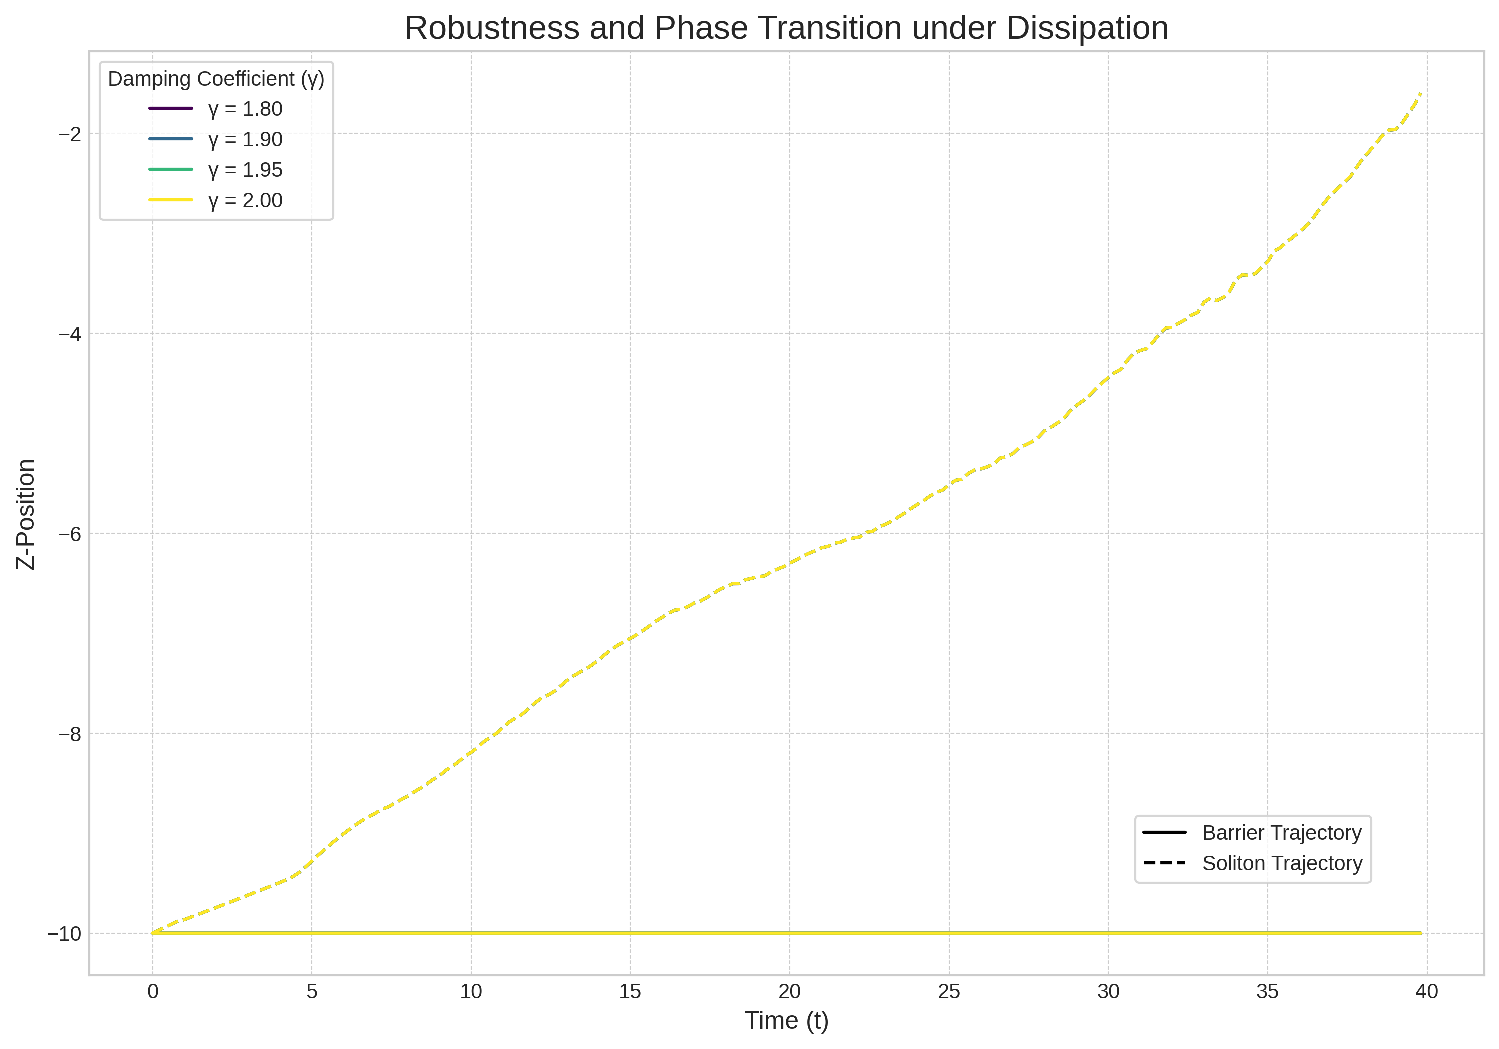
\includegraphics[width=0.9\linewidth]{fig3_dissipation.pdf}
        \caption{散逸下での頑健性と相転移。様々な減衰係数($\gamma$)に対する軌跡。$\gamma \le 1.90$ では軌跡は完全に同期するが、$\gamma \ge 1.95$ では初期位置に固定される「固定状態」へと相転移する。}
        \label{fig:dissipation}
    \end{minipage}

    \vspace{1cm} 

    % --- Figure 2 ---
    \begin{minipage}{1.0\textwidth}
        \centering
        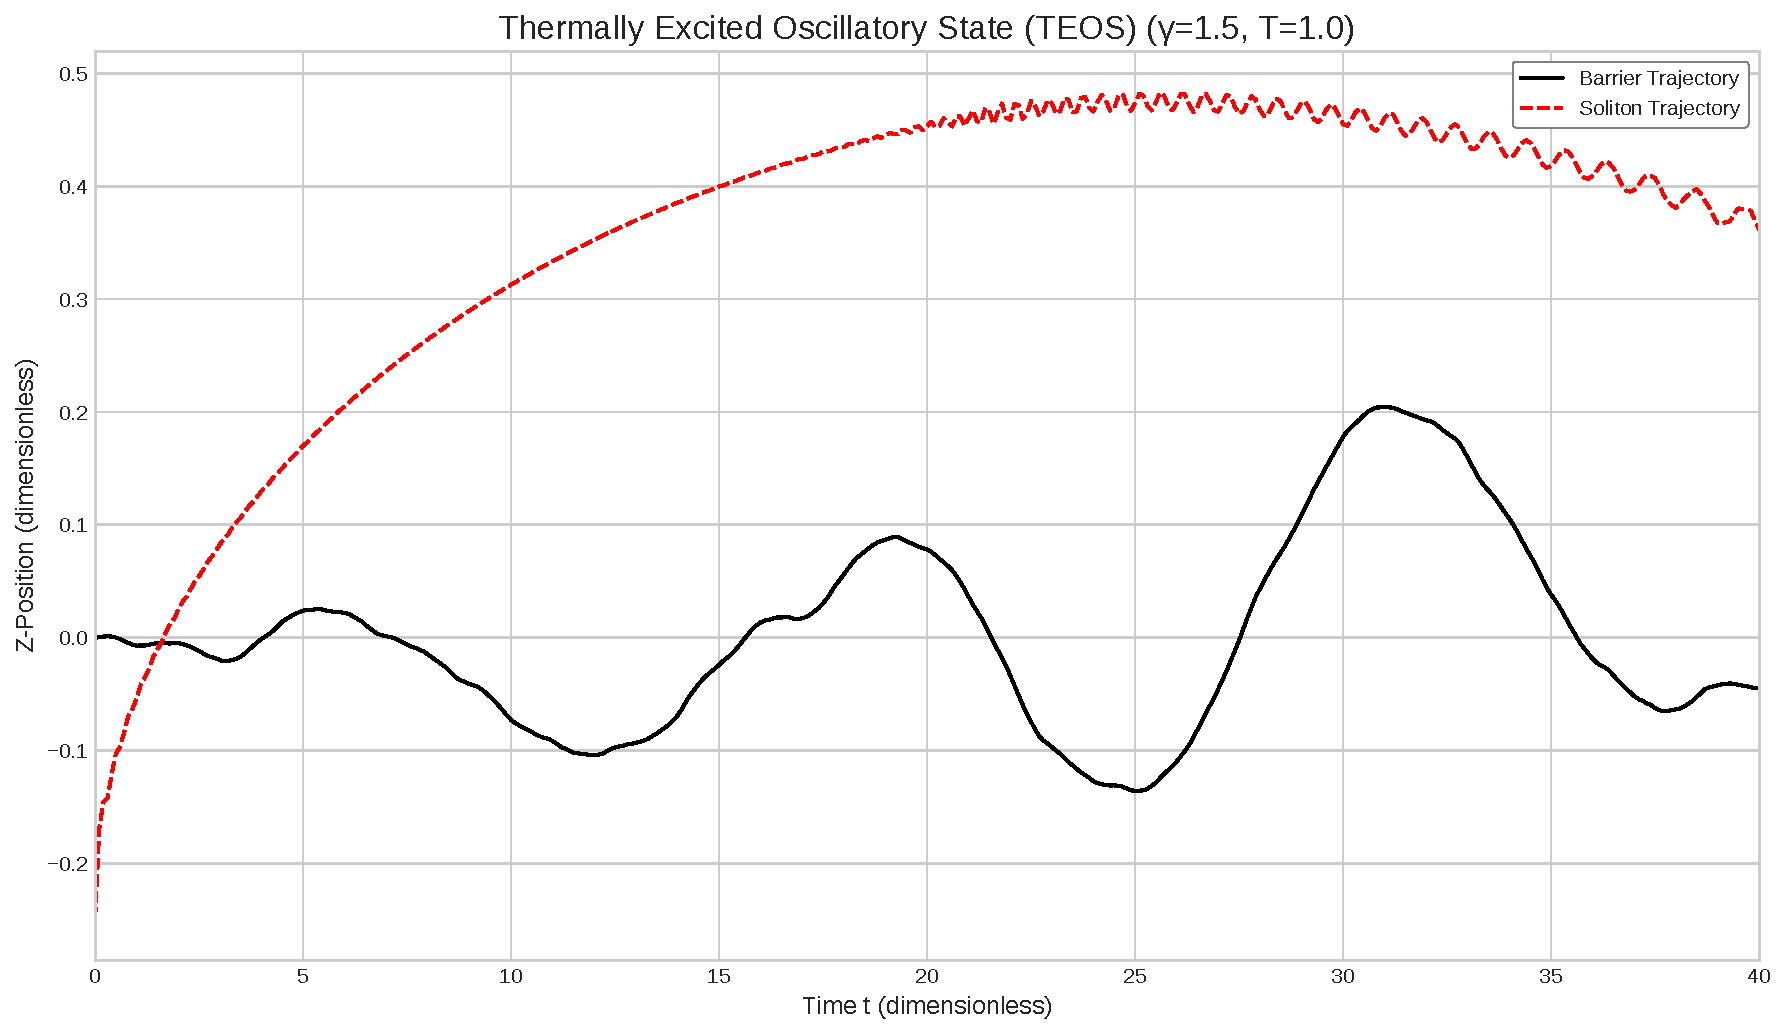
\includegraphics[width=0.9\linewidth]{fig2_TEOS_framed_thin.pdf}
        \caption{散逸と熱ゆらぎが共存する系における「熱的励起振動状態」。計算条件は、中程度の散逸($\gamma=1.5$)と強い熱ゆらぎ($T=1.0$)である。「固定状態」とは対照的に、障壁(黒実線)は持続的な振動状態を維持している。これは、熱浴からのエネルギー注入が、散逸によるエネルギー損失を補償していることを示している。}
        \label{fig:TEOS}
    \end{minipage}

\end{figure}

\begin{figure}[h!]
  \centering
  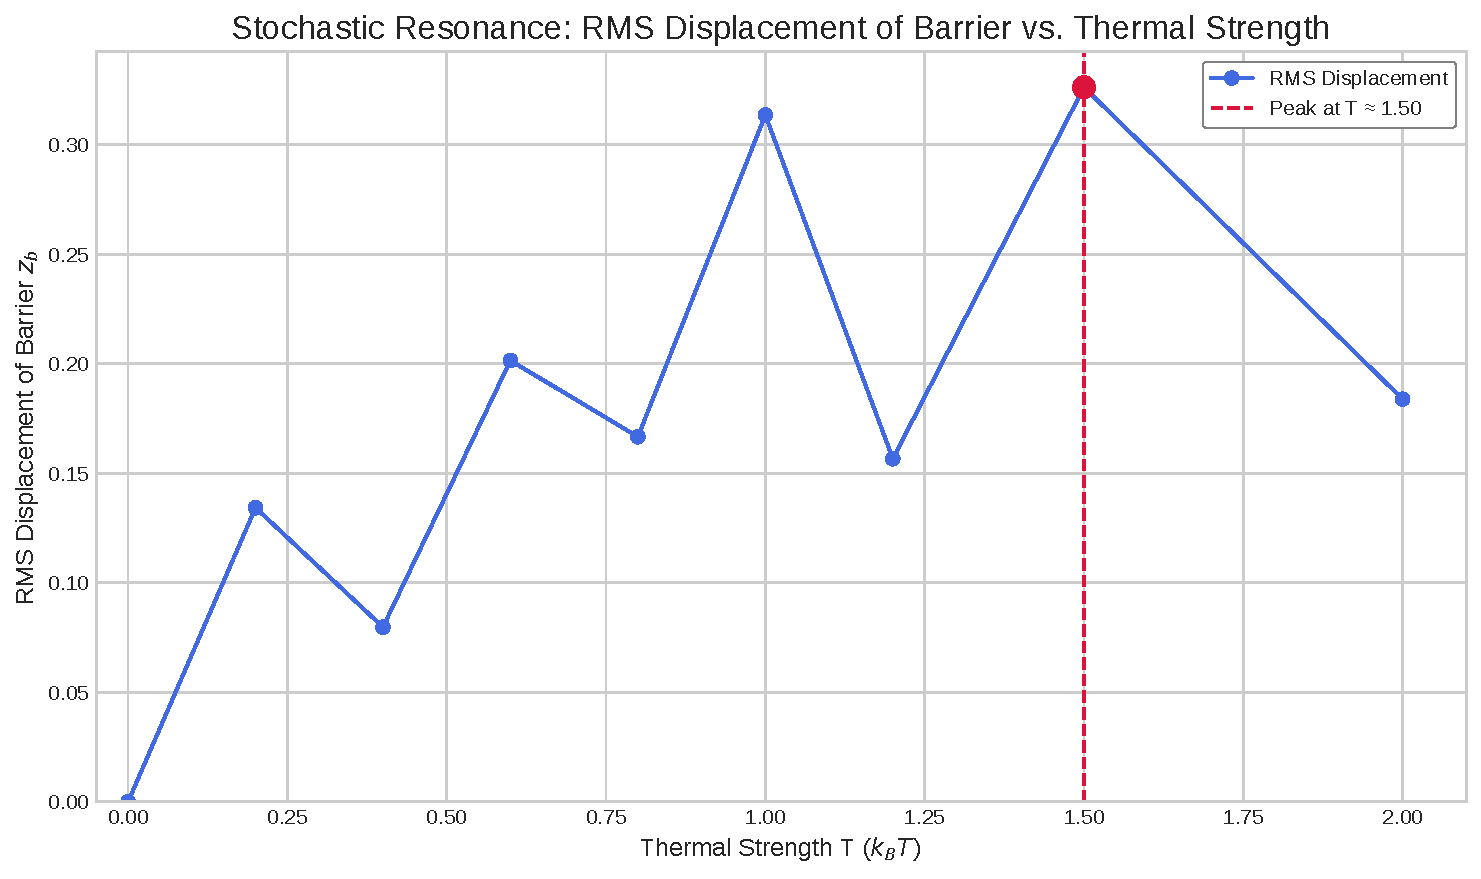
\includegraphics[width=0.9\linewidth]{stochastic_resonance_rms_framed.pdf}
  % ... (Unchanged, final version from previous turn) ...
  \caption{確率共鳴の定量的証拠。横軸は熱ゆらぎ強度$T$、縦軸は障壁の振動振幅(RMS変位)を示す。データ点は、振動振幅が$T \approx 1.5$で最大となるベル型の傾向を示しており、これは確率共鳴の特徴である。統計的な揺らぎのため曲線は凹凸を持つが、より長時間・多数回のシミュレーションにより、さらに滑らかな曲線が得られることが期待される。}
  \label{fig:SR}
\end{figure}

\FloatBarrier
\section{考察 (Discussion)}
% ... (Unchanged) ...
本研究の一連の数値シミュレーションを通じて、我々のモデルが示す3つの異なる動的状態(相)が明らかになった。すなわち、(1)理想系における「安定結合移動」、(2)強い散逸下での「固定状態」、そして(3)散逸と熱ゆらぎが共存する系での「熱的励起振動状態」である。これらの相の存在は、我々のモデルが、環境条件に応じて多様で豊かな物理現象を内包していることを示している。

特に、今回新たに見出された「熱的励起振動状態」は、物理的にも生物学的にも、深い洞察を提供する。散逸系は、外部からのエネルギー供給がなければ、やがて熱的死(このモデルでは「固定状態」)に至るのが自然な帰結である。しかし、我々のシミュレーションは、熱ゆらぎという、一見ランダムで無秩序なエネルギーが、この「死」を回避させ、系を動的な平衡状態に維持する上で、決定的な役割を果たすことを示した。

このメカニズムは、我々哺乳動物が体温を一定に保つ「恒温性(Homeostasis)」と、顕著なアナロジーを持つ。細胞内のミトコンドリアが生成する「熱」は、生命活動の背景となるだけでなく、我々のモデルが示唆するように、散逸によるエネルギー損失を補い、システム全体の活動を維持するための、能動的なエネルギー源として機能している可能性がある。この観点から見れば、「熱ゆらぎ」は単なるノイズではなく、生命がその動的な秩序を維持するために不可欠な、創造的要素と捉えることができる。

さらに、「引きずり現象」に見られる確率共鳴の兆候は、このアナロジーを一層深める。これは、熱ゆらぎ(体温)が、細胞間の微弱な信号伝達を助け、全身にわたって情報が効率的に伝播することを可能にする、という新しい仮説へと繋がる。すなわち、生命は、避けられないノイズである熱ゆらぎを、単に克服するだけでなく、むしろ情報伝達の増幅器として積極的に利用しているのかもしれない。この「ノイズに助けられた情報伝達」という描像は、細胞内のような複雑でノイジーな環境で、いかにして正確な生命活動が維持されているのかという、生物物理学の中心的な問いに、新たな光を当てるものである。

\FloatBarrier
\section{結論と将来課題 (Conclusion and Future Work)}
% ... (Unchanged) ...
本研究では、作用素環論に着想を得た、量子場と古典場が動的に結合する3次元数式モデルを拡張し、散逸と熱ゆらぎが共存する、より現実的な環境下での系のダイナミクスを検証した。その結果、散逸が引き起こす「固定状態」とは質的に異なる、新たな動的平衡状態である「熱的励起振動状態」の存在を明らかにした。この状態は、系が熱浴からのエネルギー注入によって散逸を補償するメカニズムを示しており、さらに、熱ゆらぎが量子場からの微弱な信号を増幅する「確率共鳴」の定量的な証拠も観測された。これらの結果は、我々のモデルが、生命系における恒温性や、ノイズ環境下での情報伝達といった、複雑な現象の根底にある物理的原理を捉えている可能性を示唆する。

本稿は、この「熱的励起振動状態」と「確率共鳴」という、我々が発見した新しい物理現象に関する第一報である。この新大陸の全貌を解明するため、我々は今後の研究課題として、以下の探求を計画している。
\begin{enumerate}
    \item \textbf{相図の作成:} 散逸係数$\gamma$と熱ゆらぎの強さ$T$を広範なパラメータ空間で変化させ、「安定結合移動」「固定状態」「熱的励起振動状態」が出現する領域を完全にマッピングし、系の完全な相図を作成する。
    \item \textbf{確率共鳴の定量的解析:} 観測された確率共鳴のメカニズムをさらに詳細に解析し、信号対雑音比(SNR)が最大となる条件などを特定する。
    \item \textbf{障壁の量子化:} 本研究で古典的に扱った障壁を量子化し、全ての自由度が量子力学的に記述される、完全な量子多体系としてのモデルへと拡張する。
\end{enumerate}

\section*{謝辞および AI 利用開示}
% ... (Unchanged) ...
本研究の数式設計、Pythonコード生成、シミュレーション設計および原稿整形にはOpenAI GPT、Google Geminiなどの大規模言語モデルを対話的に活用した。これらのAIツールの助力により、試行錯誤の効率化と文書校正の迅速化が実現した。

\section*{再現性とライセンス}
% ... (Unchanged) ...
本研究の公式レコードはZenodoにて公開される。DOI: \url{10.5281/zenodo.16417394}

\FloatBarrier
\appendix
\section{補遺 (Supplementary Information)}
\subsection{無次元化と物理スケール}
% ... (Unchanged) ...
本研究のシミュレーションは、現象の普遍性を探るため無次元化単位系で行われた。
\begin{quote}
\textbf{Example Mapping: スケール変換例} \\
無次元化 $\tilde t = t/t_0, \tilde{\mathbf{r}} = \mathbf{r}/\ell_0$ において、典型的なBEC実験のパラメータ(Na-23原子、$\ell_0 = 1\,\mu\text{m}$, $t_0 = 1\,\text{ms}$)を仮定した場合、シミュレーション時間 $t=40.0$ は実時間で 40 ms に相当する。本稿ではボルツマン定数 $k_B=1$ と規格化しており、このスケールでは無次元温度 $T=1.0$ は実温度約250 nKに相当する。
\end{quote}

\subsection{数値計算手法と誤差評価}
時間発展には標準的なSplit-step Fourier法を用い、計算空間には全方向に周期境界条件を課した。(計算格子サイズ: $N_x=N_y=64, N_z=256$)。

\begin{figure}[h!]
  \centering
  \includegraphics[width=0.9\linewidth]{fig_S1_conservation.pdf}
  \caption*{図S1: 理想系におけるエネルギーと粒子数の保存誤差。}
  \label{fig:s1_ideal}
\end{figure}

\begin{figure}[h!]
  \centering
  \includegraphics[width=0.9\linewidth]{fig_S2_mass_effect.pdf}
  \caption*{図S2: 有効質量(M)が系のダイナミクスに与える影響。}
  \label{fig:s2_mass}
\end{figure}

\begin{figure}[h!]
  \centering
  \includegraphics[width=0.9\linewidth]{conservation_law_thermal.pdf}
  % ★★★ ここからが修正箇所 ★★★
  \caption*{図 S3: 熱ゆらぎ存在下での保存則の検証 (γ = 1.5, T = 1.0) (左 Y 軸) 全エネルギーの初期値からの偏差 ΔE(t)。(右 Y 軸) 粒子数の初期値 (N=1) からの偏差。Split-step Fourier 法の数値誤差の累積により、粒子数には僅かなドリフトが見られるものの、その偏差は10⁻¹¹という極めて小さいオーダーに収まっており、本計算手法が高い安定性を持つことを示している。}
  % ★★★ ここまでが修正箇所 ★★★
  \label{fig:s3_thermal}
\end{figure}

\FloatBarrier
\begin{thebibliography}{9}
\bibitem{feynman} R. P. Feynman, \textit{Phys. Rev.} \textbf{56}, 340 (1939).
\bibitem{ingber} D. E. Ingber, \textit{J. Cell Sci.} \textbf{104}, 613 (1993).
\bibitem{fleck} J. A. Fleck Jr., J. R. Morris, and M. D. Feit, \textit{Appl. Phys.} \textbf{10}, 129 (1976).
\bibitem{kane} C. L. Kane and E. J. Mele, \textit{Phys. Rev. Lett.} \textbf{95}, 146802 (2005).
\end{thebibliography}

\end{document}